\paragraph{}El usuario administrador de centro puede realizar consultas sobre
los departamentos, titulaciones, asignaturas, asesores y sobre los alumnos que
existan en el sistema. Además también puede realizar consultar de datos
históricos referentes a esta misma información en diferentes cursos académicos.

\paragraph{}La figura \ref{diagramaNivel3-ExplotacionSistema-adminCentro}
muestra el nivel de abstracción 3: Explotación del sistema (módulo Administrador
de centro).

  \begin{figure}[!ht]
    \begin{center}
      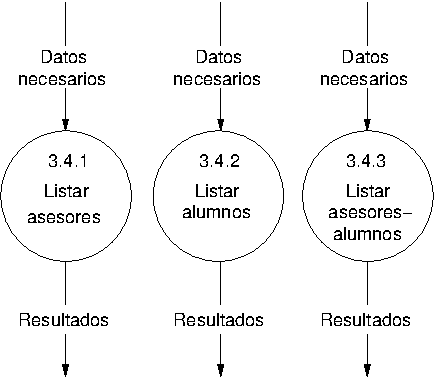
\includegraphics[]{08.Analisis_Funcional/8.2.DFDs/Niveles/Nivel3/AdministradorCentro/ExplotacionSistema/Diagramas/nivel3-ExplotacionSistema.pdf}
      \caption{Nivel de abstracción 3: Explotación del sistema (módulo
      Administrador de centro).}
      \label{diagramaNivel3-ExplotacionSistema-adminCentro}
    \end{center}
  \end{figure}
